% Generated by support/export-artifacts.py; do not edit.
% Slug: ch71-padding
% Source: chapters/ch71.tex:33
% TikZ source: chapters/ch71.tex:35
% Original label: \label{fig:ch71-padding}
% Original caption (LaTeX source):
%   Offsets describe native storage, including padding that carries no field value.
% Caption: Offsets describe native storage, including padding that carries no field value.
% Setup: support/compiler-pseudocode.sty (TikZ libraries and shared styles).
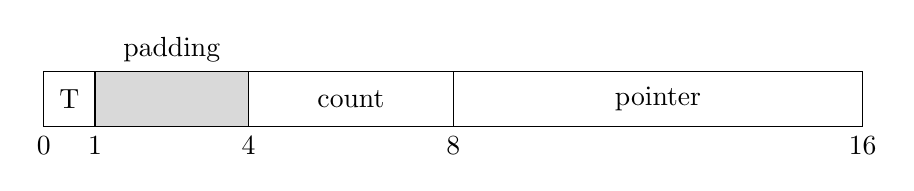
\begin{tikzpicture}[x=0.65cm,y=1cm]
\draw (0,0) rectangle (1,0.7);
\draw[fill=black!15] (1,0) rectangle (4,0.7);
\draw (4,0) rectangle (8,0.7); \draw (8,0) rectangle (16,0.7);
\node at (0.5,0.35) {T}; \node at (6,0.35) {count}; \node at (12,0.35) {pointer};
\foreach \x in {0,1,4,8,16} \node[below] at (\x,0) {\x};
\node[above] at (2.5,0.7) {padding};
\end{tikzpicture}

% Original figure LaTeX:
% \begin{figure}[htbp]
% \centering
% \begin{tikzpicture}[x=0.65cm,y=1cm]
% \draw (0,0) rectangle (1,0.7);
% \draw[fill=black!15] (1,0) rectangle (4,0.7);
% \draw (4,0) rectangle (8,0.7); \draw (8,0) rectangle (16,0.7);
% \node at (0.5,0.35) {T}; \node at (6,0.35) {count}; \node at (12,0.35) {pointer};
% \foreach \x in {0,1,4,8,16} \node[below] at (\x,0) {\x};
% \node[above] at (2.5,0.7) {padding};
% \end{tikzpicture}
% \caption{Offsets describe native storage, including padding that carries no field value.}
% \label{fig:ch71-padding}
% \end{figure}
